\documentclass{beamer}
\usepackage{graphics}
\usepackage[autoplay,autoresume,loop]{animate}
\usepackage{subcaption}
\usepackage{pgfpages}
\usepackage{longtable}


\setbeameroption{show notes on second screen=right} % Both
\setbeamertemplate{note page}{\pagecolor{yellow!5}\insertnote}\usepackage{palatino}

\usetheme{metropolis}           % Use metropolis theme
\title{Fake News Detection Using Machine Learning}
\date{September 10, 2019}
\author{Author: Simon Lorent \\ Supervisor: Aswhin Ittoo}
\institute{University Of Li\`ege}
\begin{document}
  \maketitle
  \section{Introduction}

  \begin{frame}{Fake news used to influence elections}
  2016 US presidential elections (Allcott et al.)\cite{Allcott2017}
	  \begin{itemize}
	 \item $62\%$ of US citizens get their news for social medias\cite{gottfried2016news}
	 \item Fake news had more share on Facebook than mainstream news\cite{silverman2016teens}.
	\end{itemize}
	\note[item]{Expliquer l'inpact des fake news sur les elections}
	\note[item]{La suite définit ce que sont les fake news}
  \end{frame}

  \begin{frame}{Definition}
  \newtheorem{def:fake_news}{Definition}
	\begin{def:fake_news}
	Fake news is a news article that is intentionally and verifiable false\cite{shu2017fake}
	\end{def:fake_news}
	\note[item]{Dire que l'on peut caracteriser les fake news de plusieurs façon: le contenu et le context}
  \end{frame}

  \begin{frame}[allowframebreaks]{Fake News Characterisation}
News content features:
  	\begin{itemize}
		 \item \textbf{Source}: Where does the news come from, who wrote it, is this source reliable or not.
		 \item \textbf{Headline}: Short summary of the news content that try to attract the reader.
		 \item \textbf{Body Text}: The actual text content of the news.
		 \item \textbf{Image/Video}: Usualy, textual information is agremented with visual information such as images, videos or audio.  
		\end{itemize}
	\note{}
	\newpage
	\vfill
	\begin{figure}
		 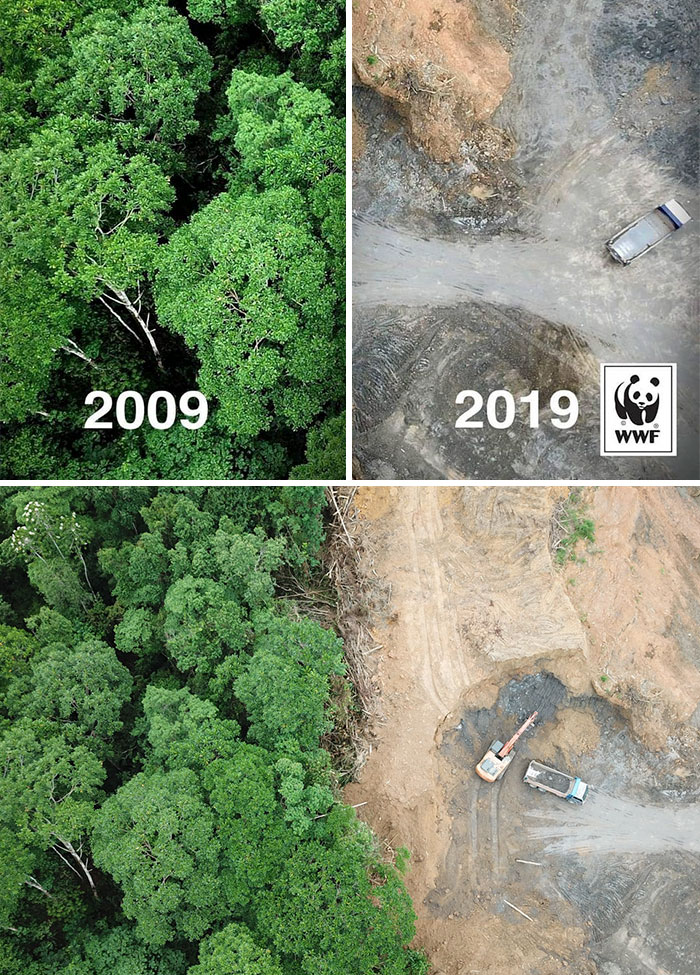
\includegraphics[scale=0.20]{fake-news-photos-viral-photoshop-8-5c6fe61f88240__700}
	\end{figure}
	\newpage
  Different kind of models:
	  	\begin{itemize}
		 \item \textbf{Expert-oriented}: relies on experts, such as journalists or scientists, to assess the news content.
		 \item \textbf{Crowdsourcing-oriented}: relies on the wisdom of crowd that says that if a sufficiently large number of persons say that something is false or true then it should be.
		 \item \textbf{Computational-oriented}: relies on automatic fact checking, that could be based on external resources such as DBpedia.
		\end{itemize}
		\note{}
	\end{frame}
	\section{Methodology}
	\begin{frame}[allowframebreaks]{Methodology}
		Goal:
		\begin{itemize}
			\item Comparing the performances of "traditional" machine learning techniques and deep learning techniques
			\item Comparing the performances of these techniques on two differents datasets.
		\end{itemize}
		\note{}
		\newpage
		Models used:
		\begin{itemize}
			\item Na\"ive-Bayes
			\item SVM
			\item Decision Tree
			\item Ridge Classifier
			\item LSTM
			\item Attention Mechanism\cite{zhou-etal-2016-attention}
		\end{itemize}
		\note{}
	\end{frame}
	\begin{frame}[allowframebreaks]{Attention Mechanism}
		\begin{figure}
		 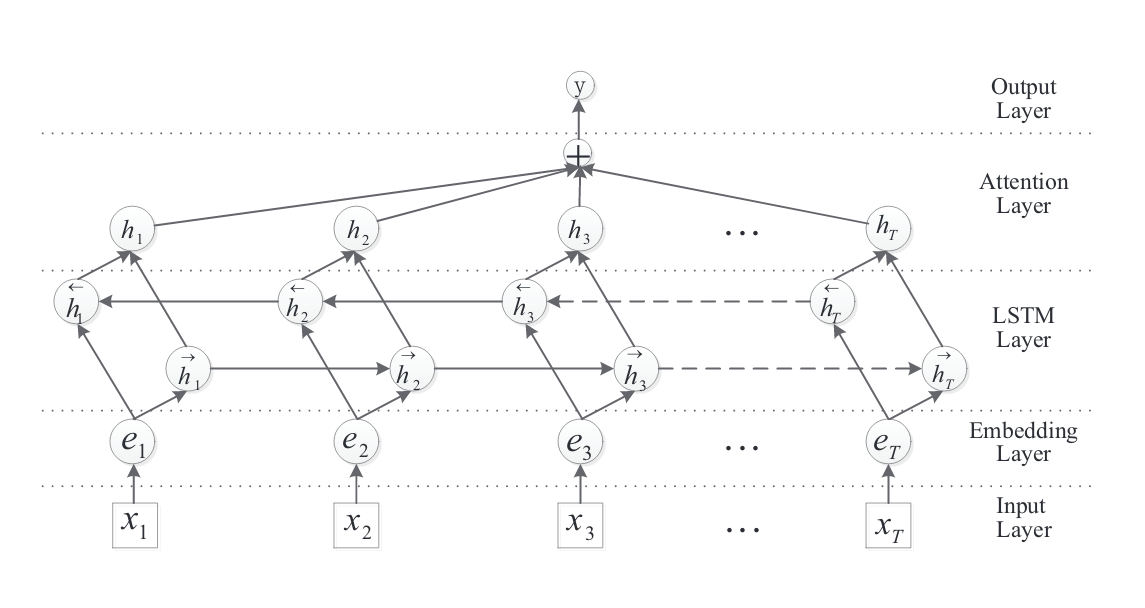
\includegraphics[scale=0.25]{attention}
	\end{figure}
	\note{}
	\end{frame}
	\begin{frame}{Word Embedding}
		\begin{itemize}
			\item One-hot encoding 
			\item Word2Vec\cite{Mikolov2013}
		\end{itemize}
		\begin{itemize}
			\item $e_i = W_e * x_i$
			\item $e_i = $ dictionary lookup
		\end{itemize} 
		\note{$W_e$ is a tunnable parameters and word2vec are pretrained}
		\note{One-hot vector are made from the training set by building a dictionary}
	\end{frame}
	\begin{frame}{Attention Mechanism}
		\begin{equation}
			 H = [h_1,h_2,...,h_T]
		\end{equation}
		Where T is the sequence length. 
		Then we define 
		\begin{align}
		 M &= \tanh(H)\\
		 \alpha &= softmax(w^TM) \\
		 r &= H \alpha^T 
		\end{align}
		Finally, we compute $h^* = \tanh(r)$.
	\end{frame}
	\section{Results}
	\begin{frame}{Machine learning}
		\begin{figure}
		\centering
			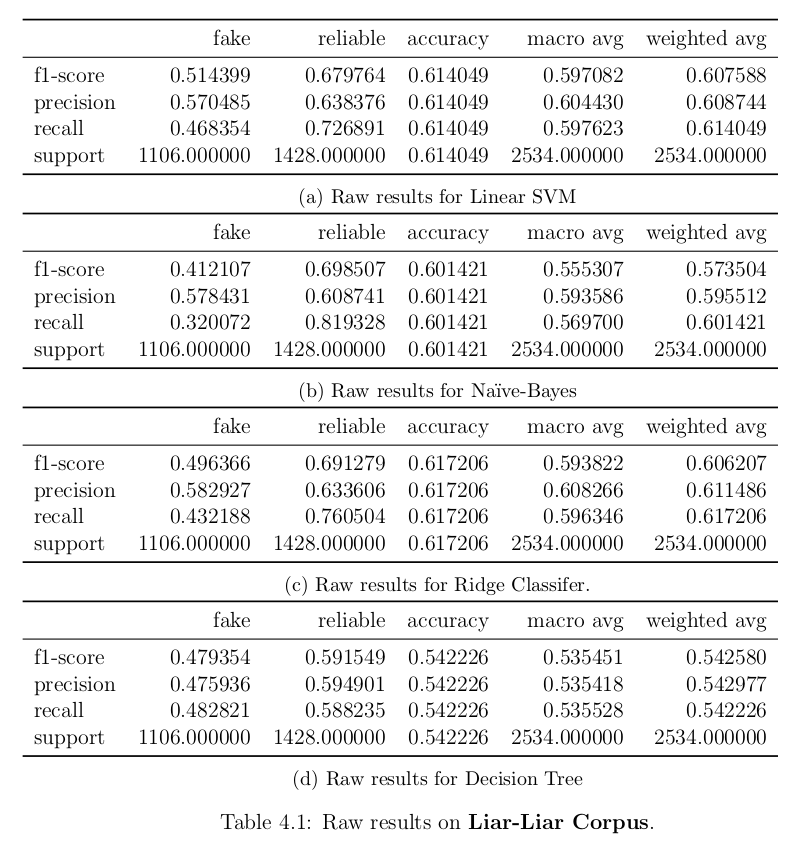
\includegraphics[width=0.6\textwidth]{res1.png}
		\end{figure}
	\end{frame}
	\begin{frame}{Machine learning II}
		\begin{figure}
		\centering
			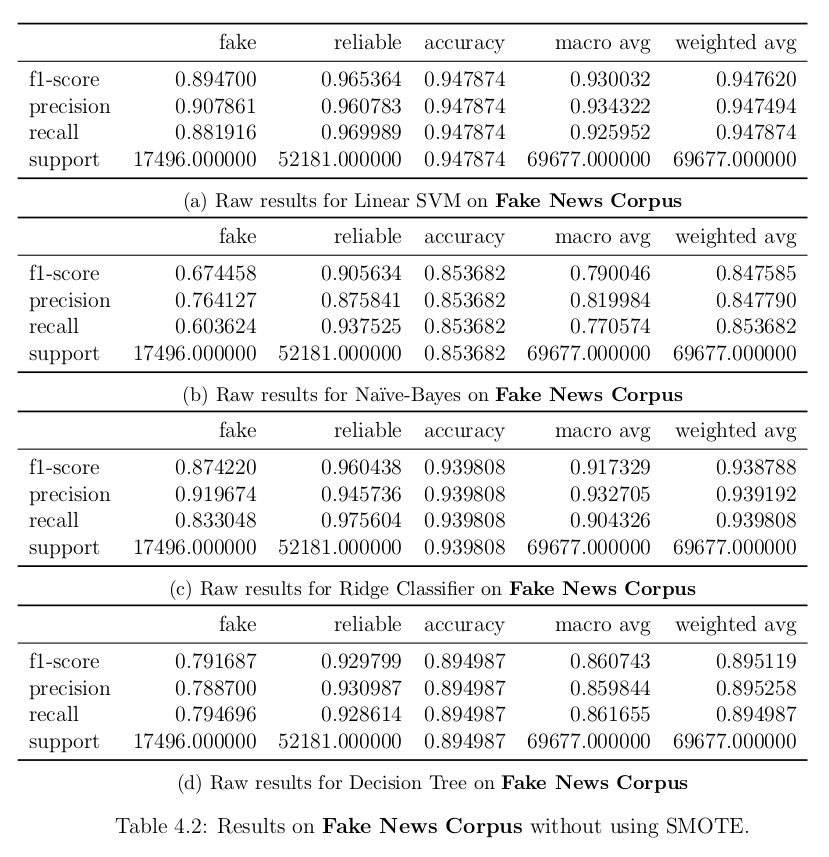
\includegraphics[width=0.6\textwidth]{res2.png}
		\end{figure}
		
	\end{frame}
	\begin{frame}{Machine learning III}
	\subsection{Deep learning}
	\begin{figure}
		\centering
			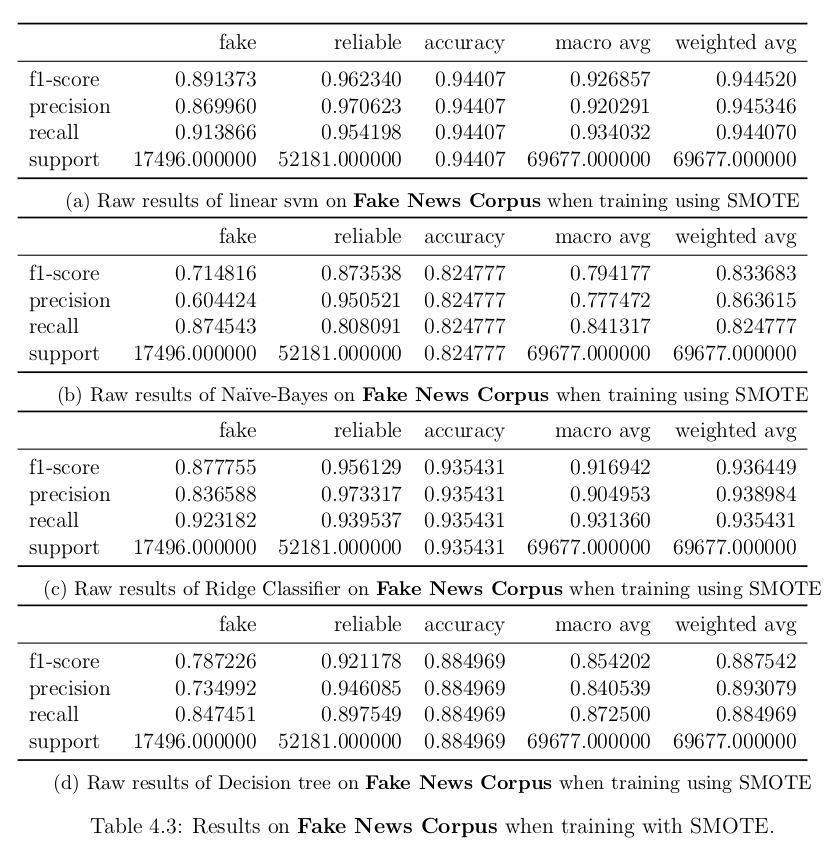
\includegraphics[width=0.6\textwidth]{res3.png}
		\end{figure}
	\end{frame}
	\begin{frame}{LSTM}
		\begin{figure}
			\centering
			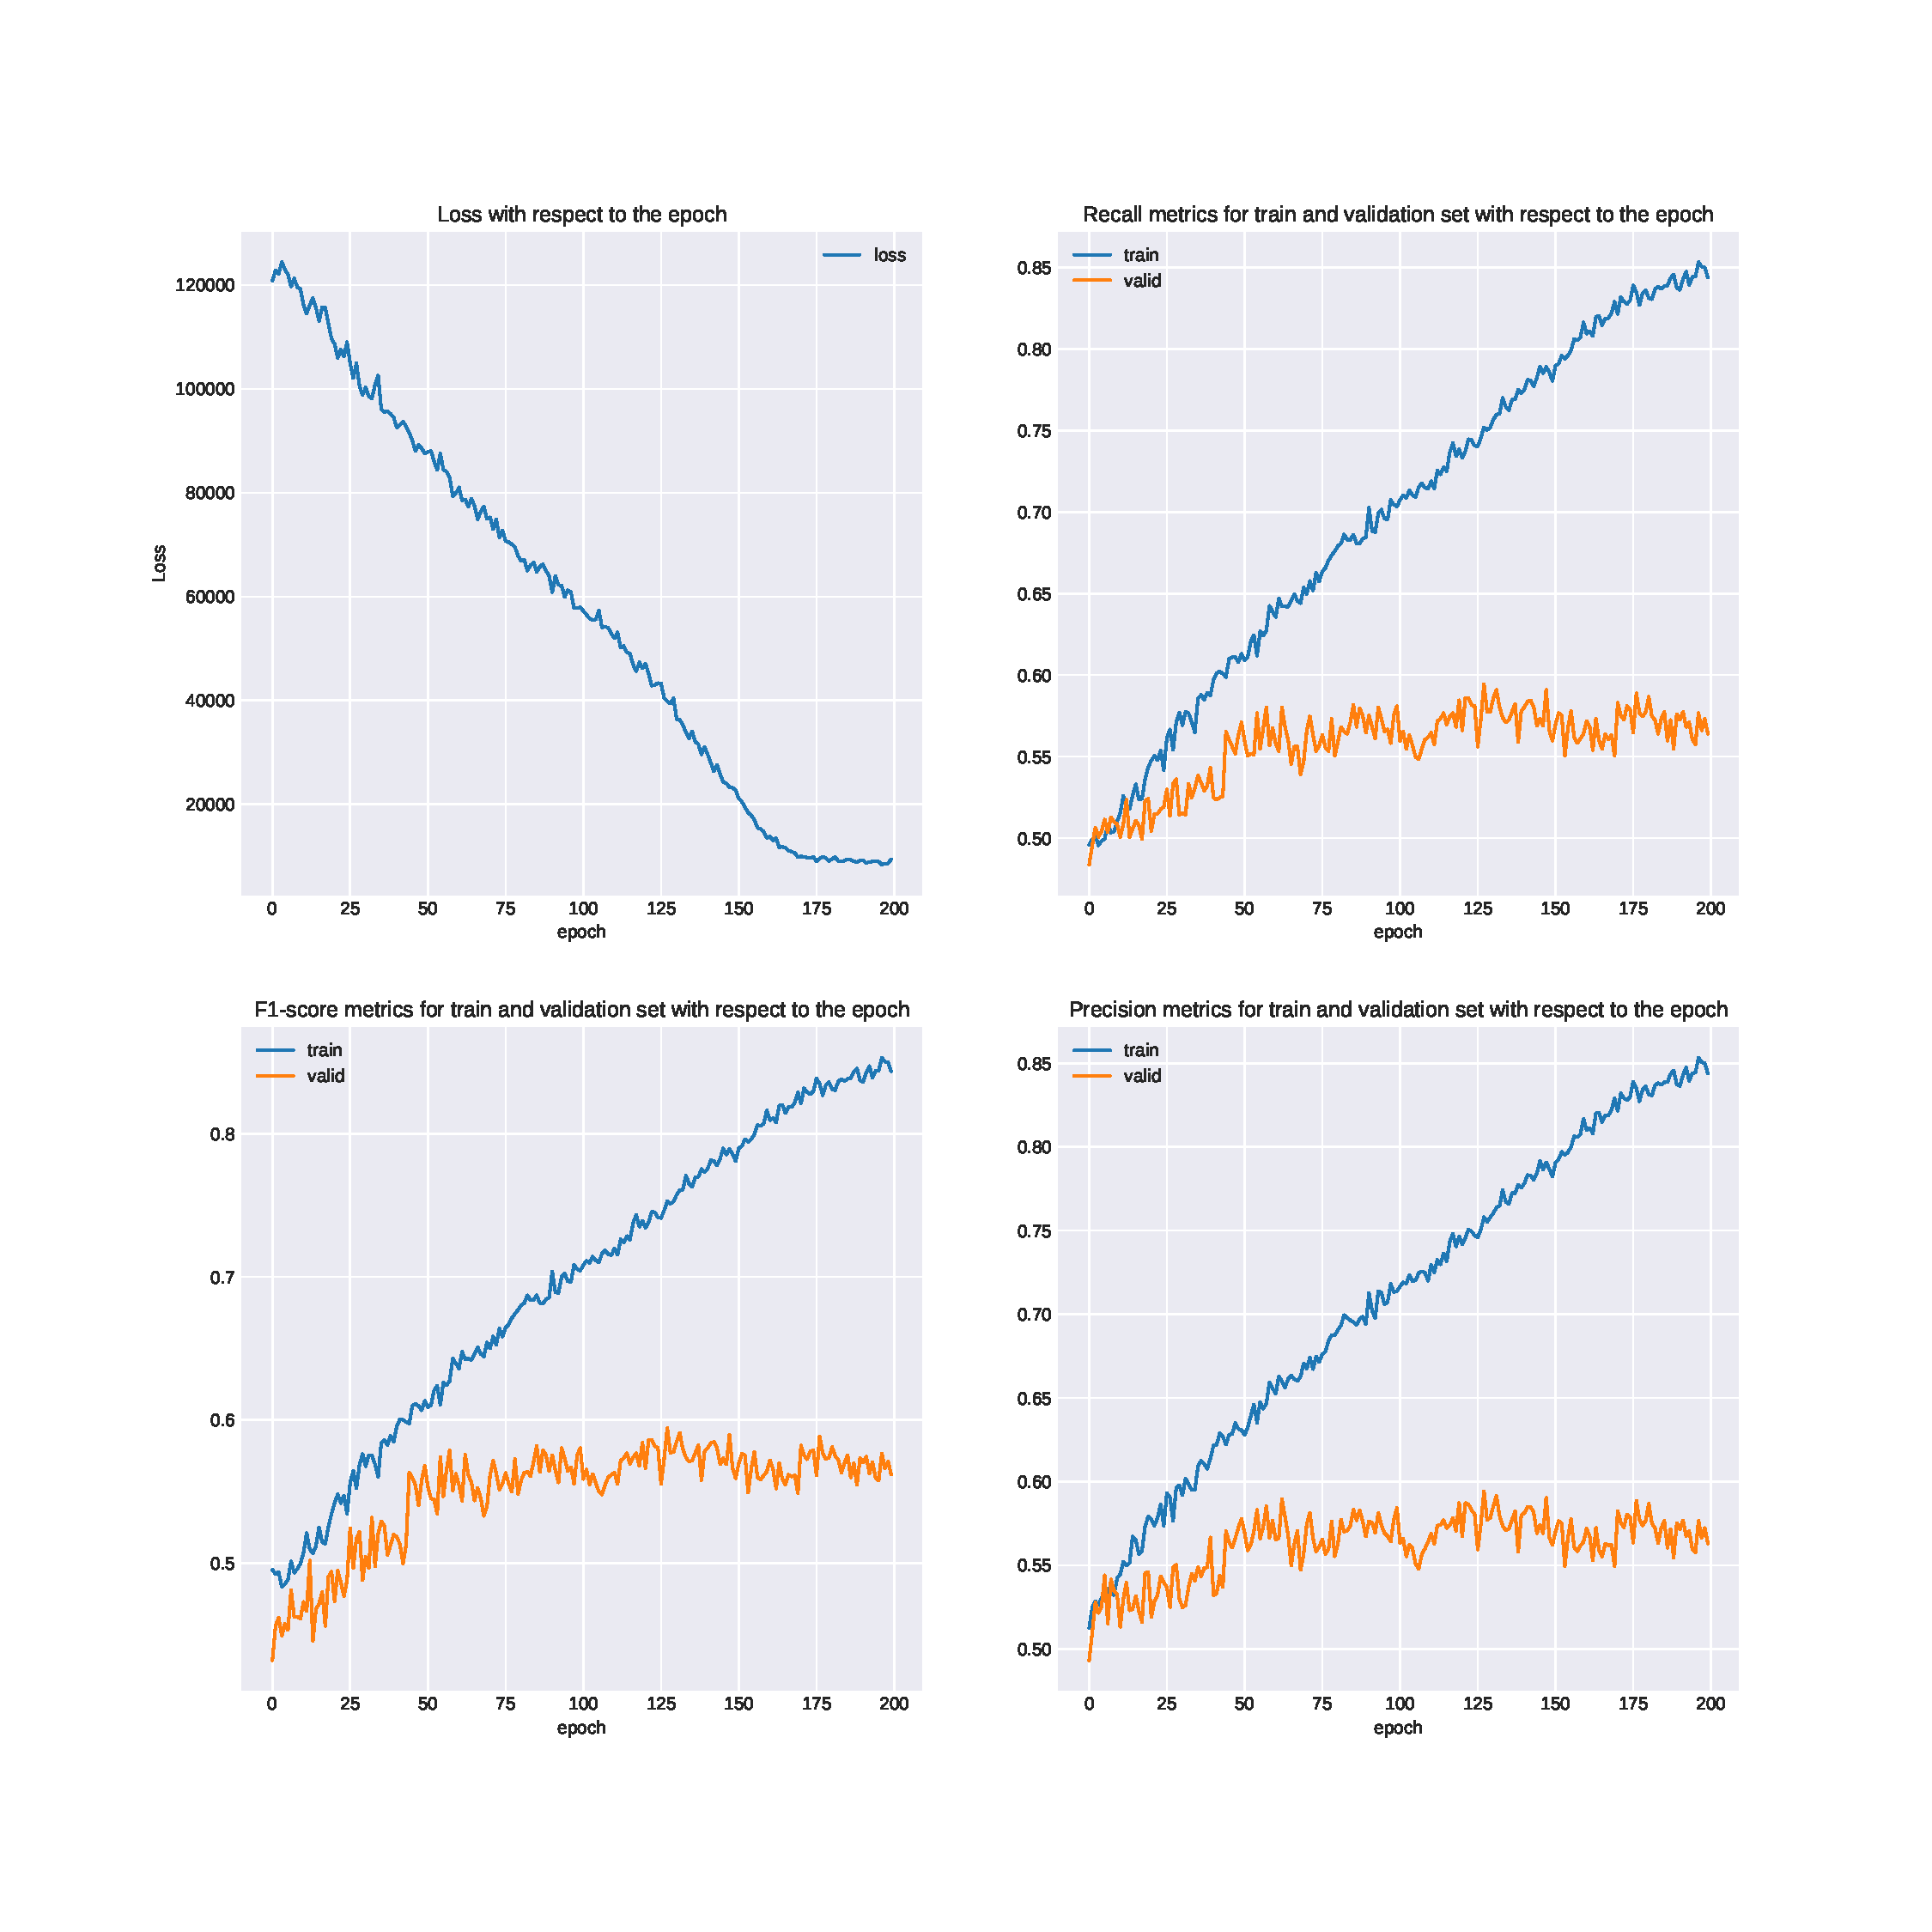
\includegraphics[width=0.6\textwidth]{lstm1.pdf}
		\end{figure}
	\end{frame}
	\begin{frame}{LSTM + word2vec}
	\begin{figure}
			\centering
			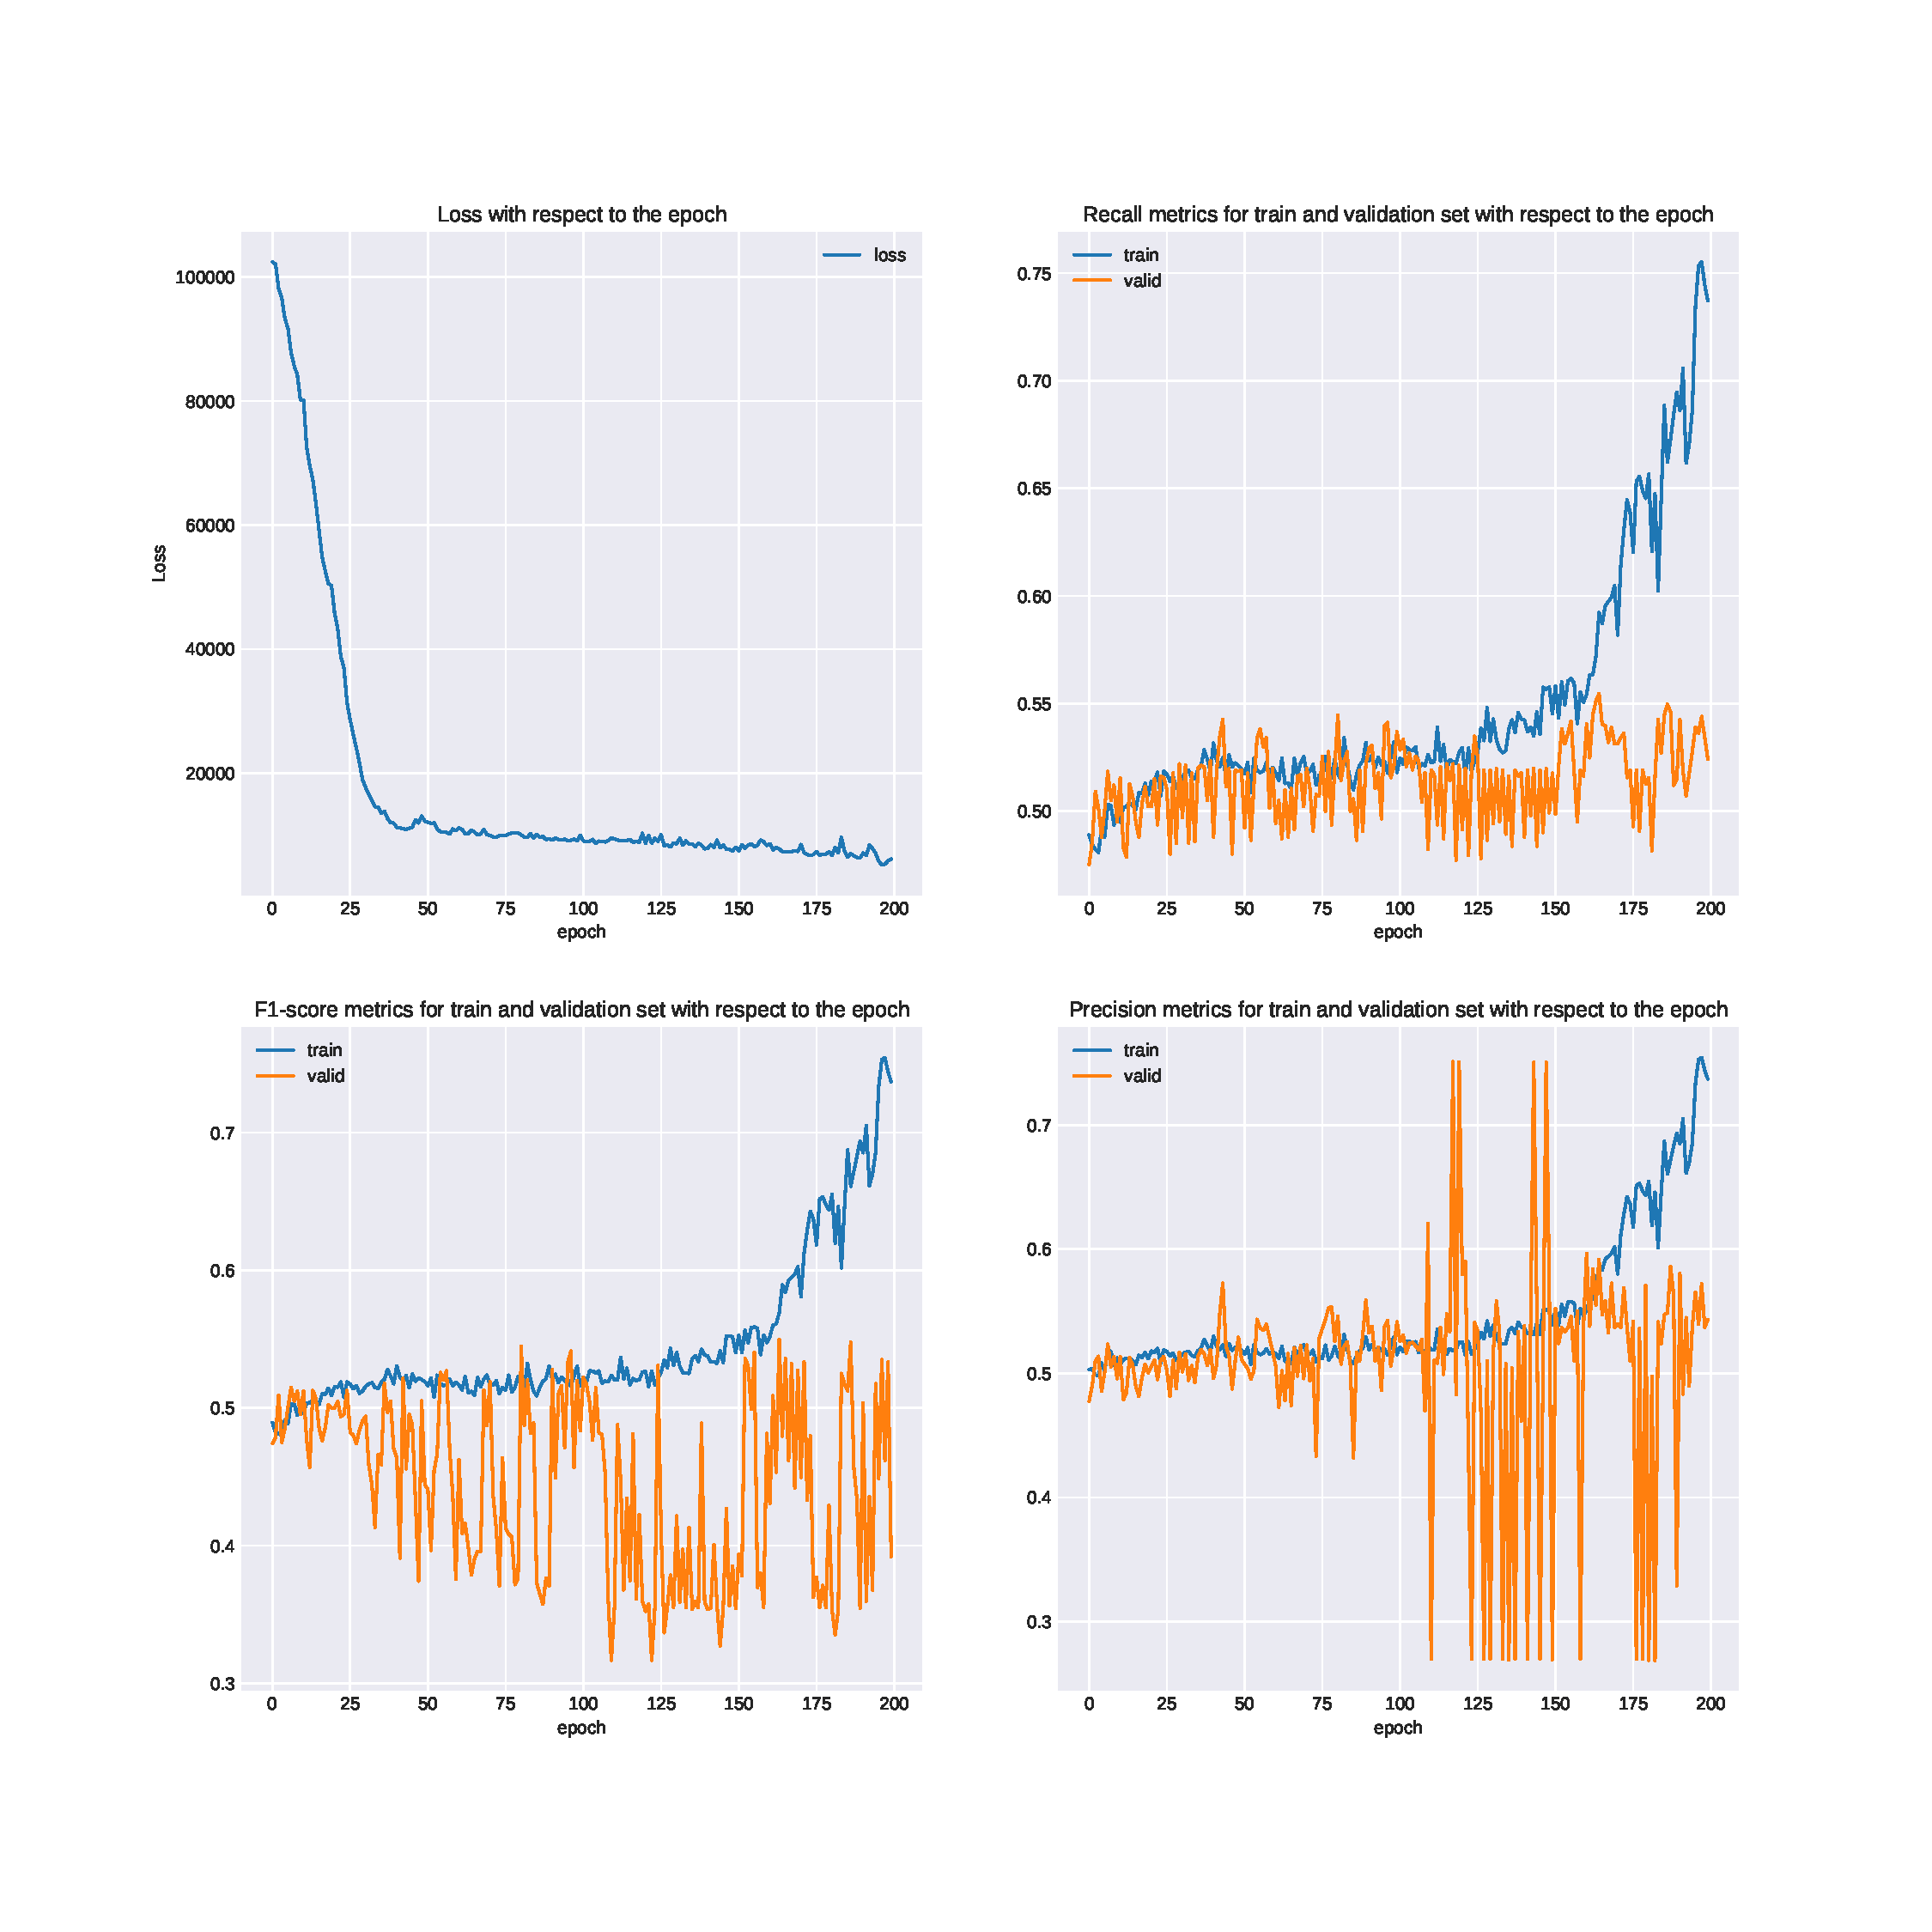
\includegraphics[width=0.6\textwidth]{lstm2.pdf}
		\end{figure}
	\end{frame}
	\begin{frame}{Attention Mechanism}
		\begin{figure}
			\centering
			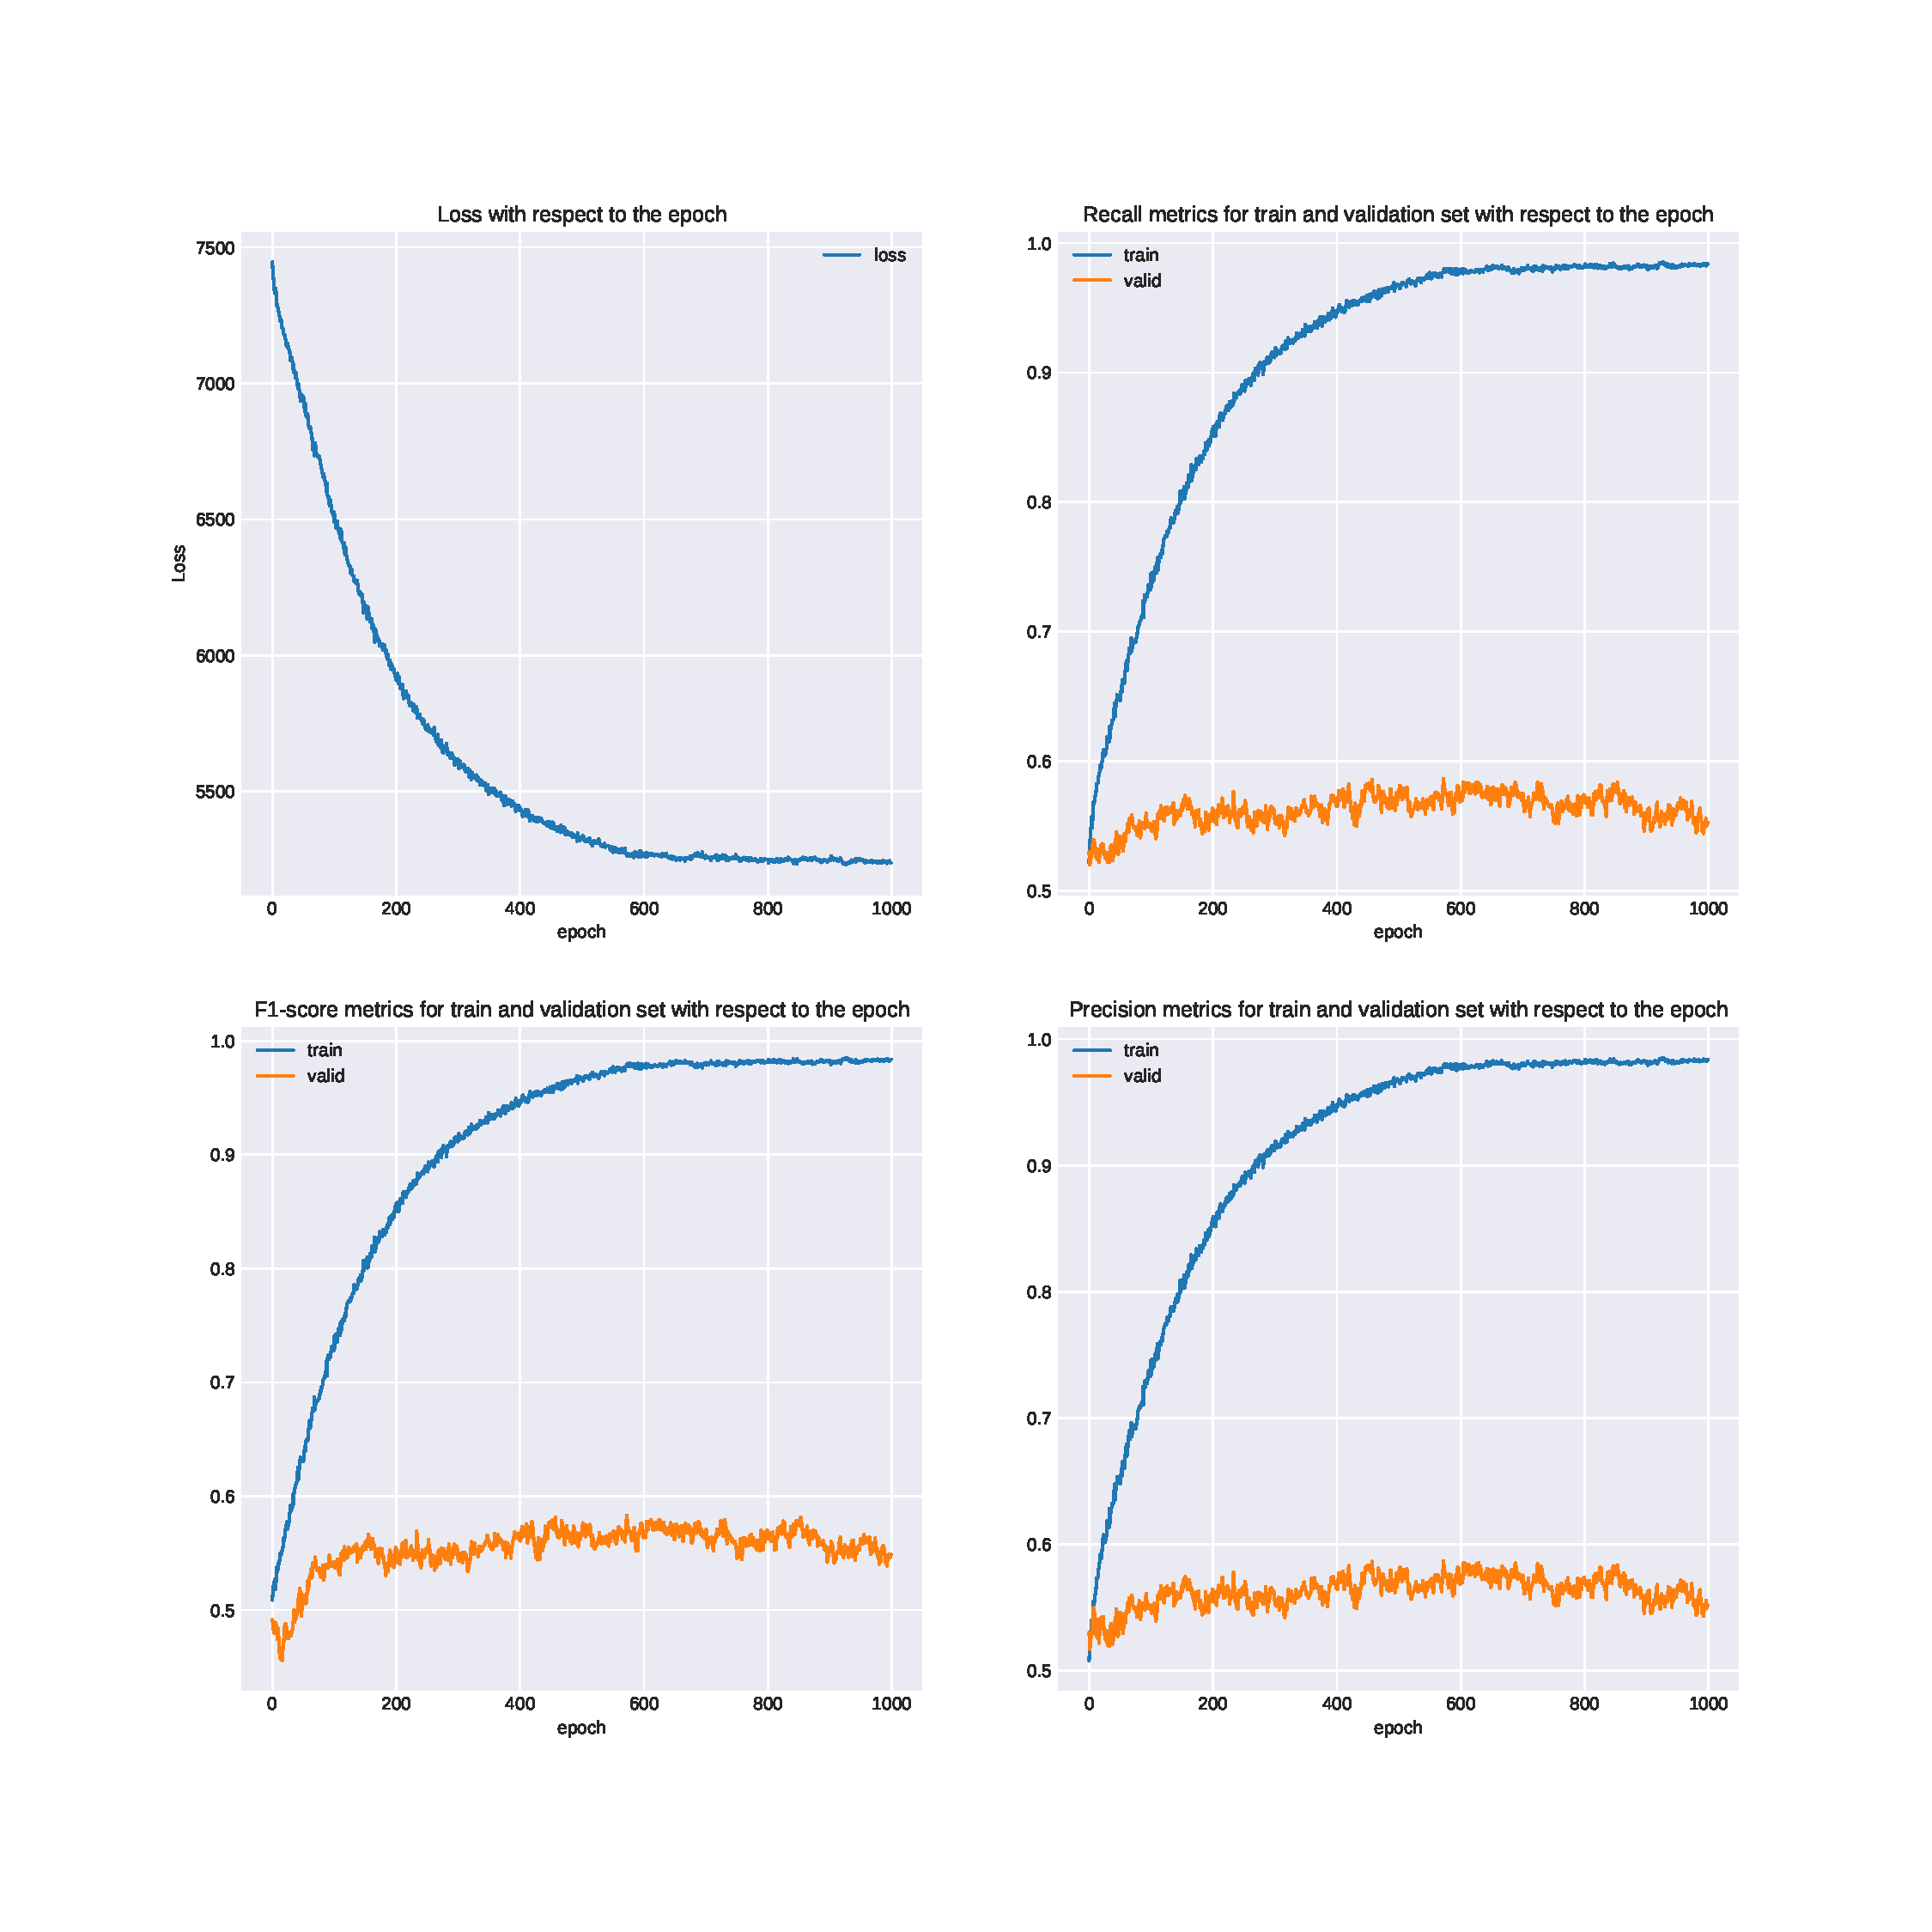
\includegraphics[width=0.6\textwidth]{attention3.pdf}
		\end{figure}
	\end{frame}
	\begin{frame}{Attention Mechanism + word2vec}
	\begin{figure}
			\centering
			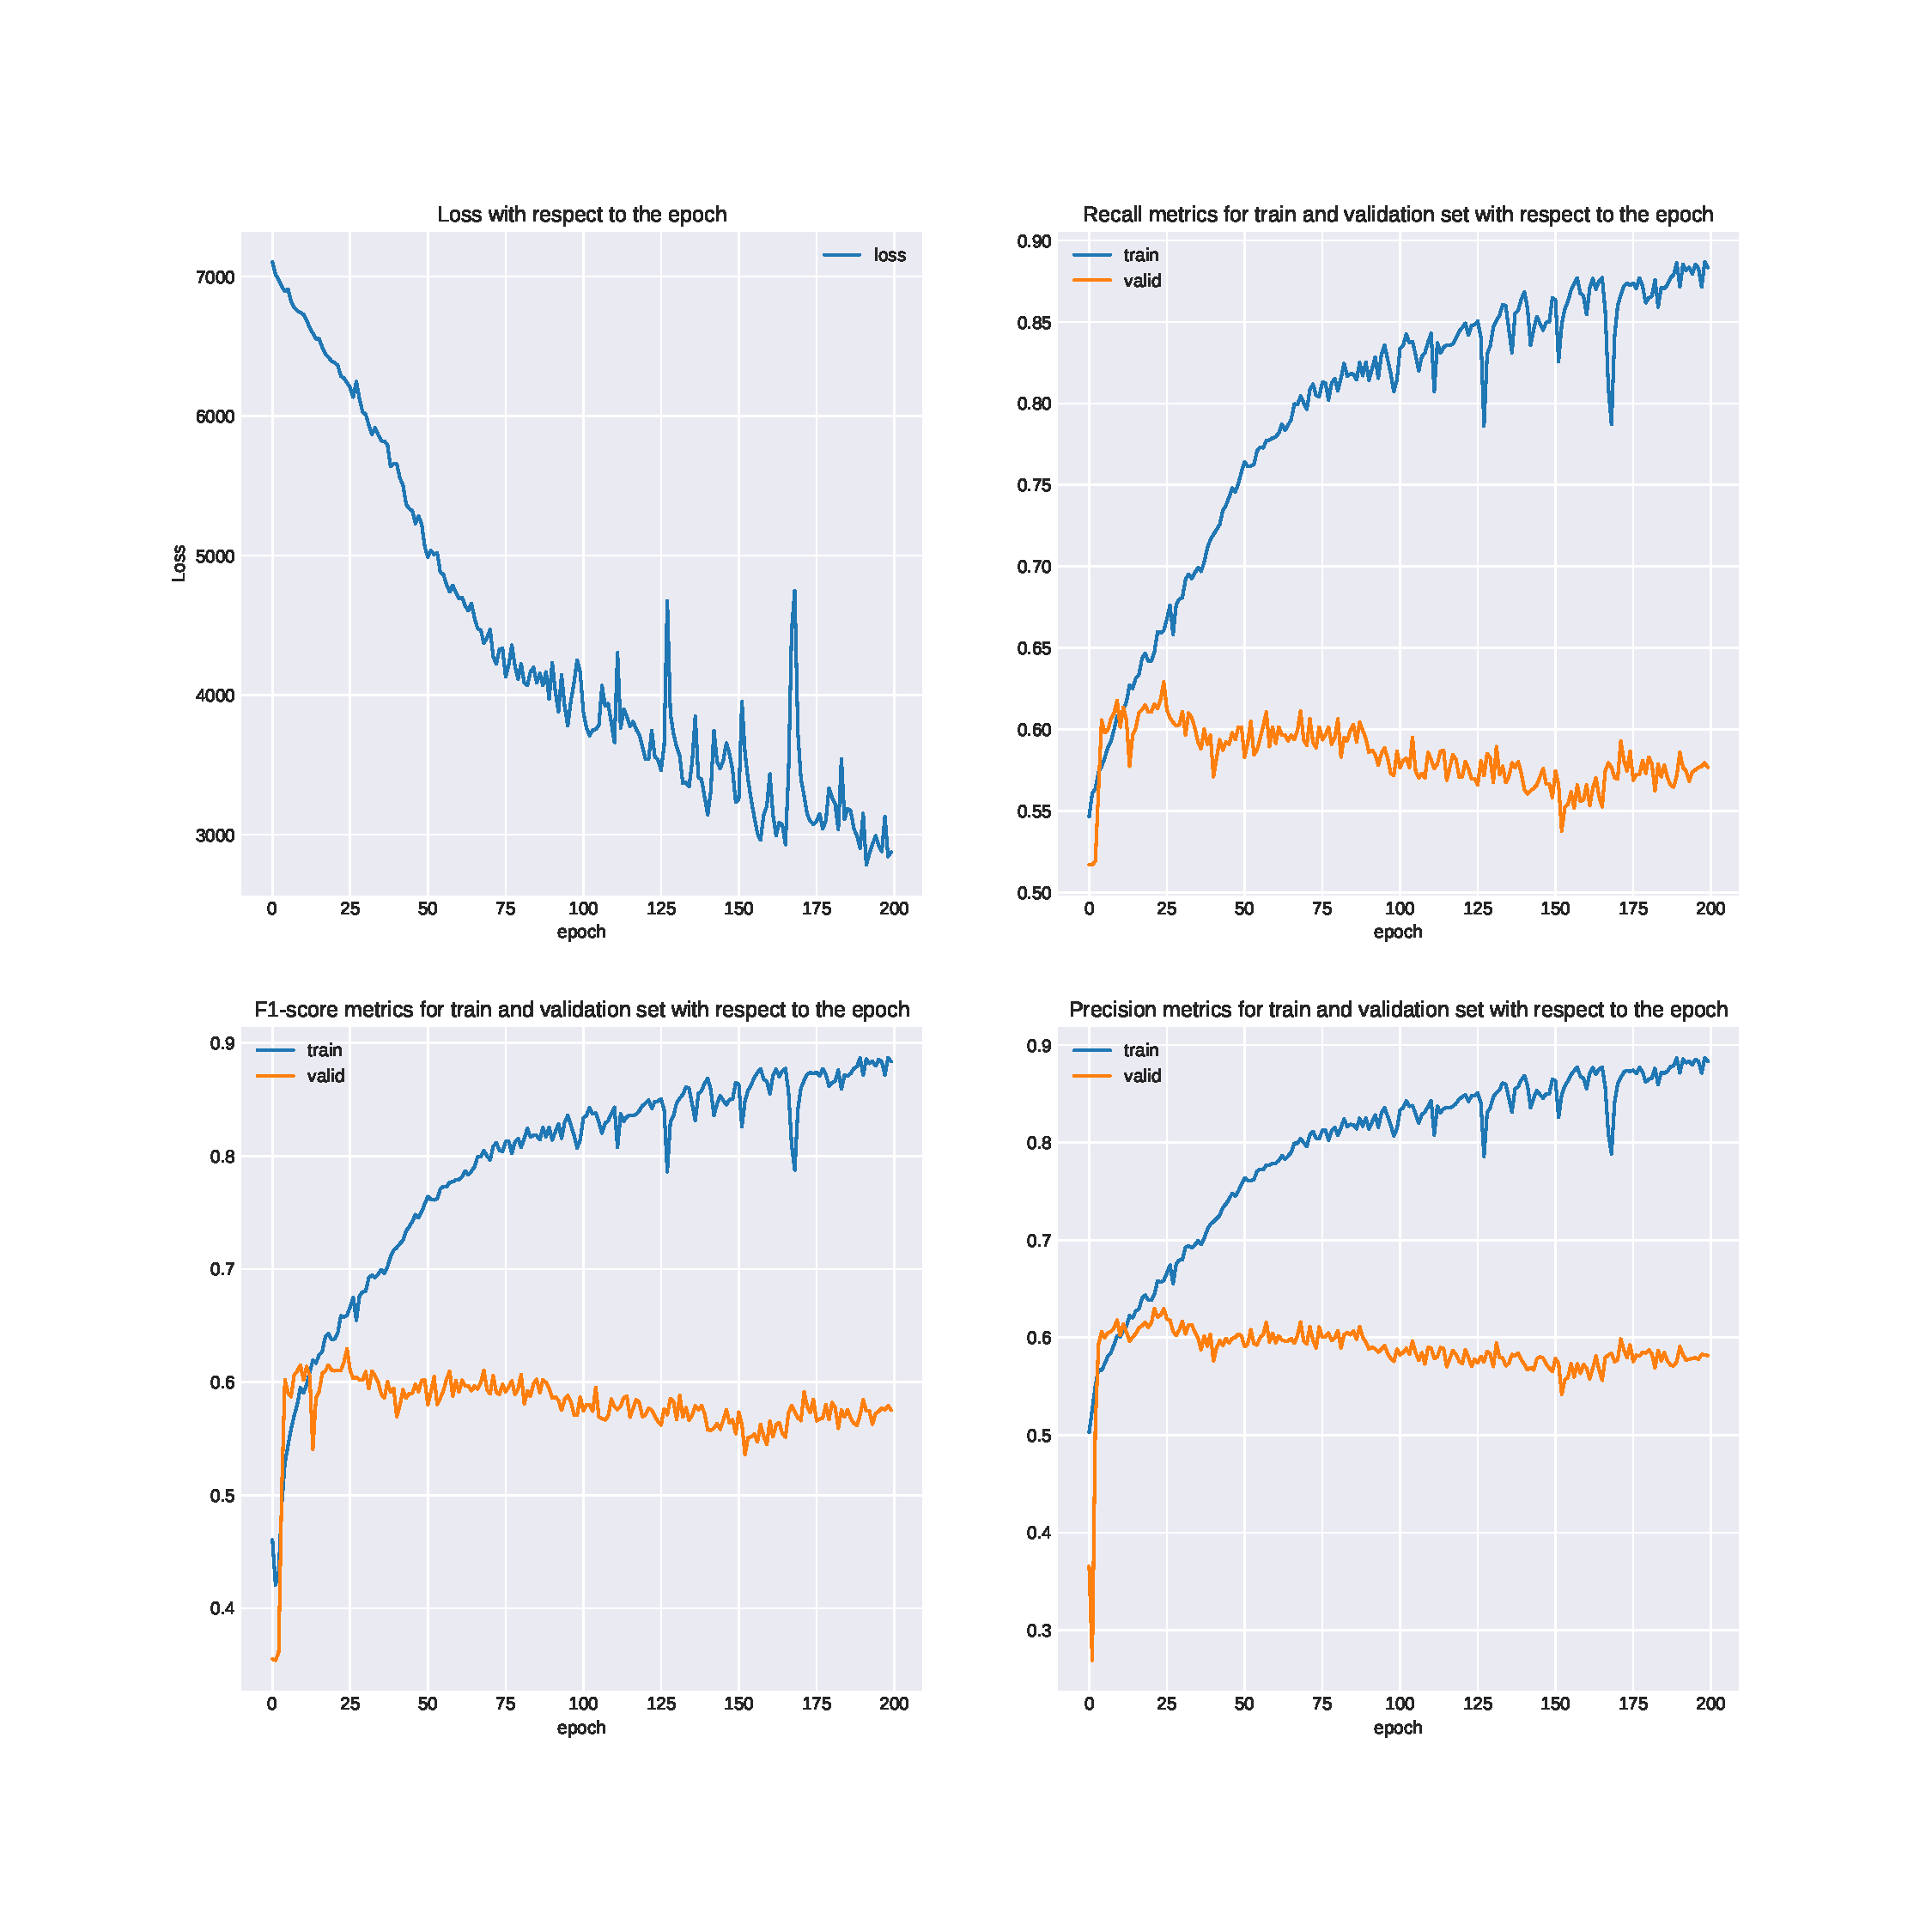
\includegraphics[width=0.6\textwidth]{attention1.pdf}
		\end{figure}
	\end{frame}
	\begin{frame}{Liar-Liar corpus results}
		\begin{figure}
		\centering
			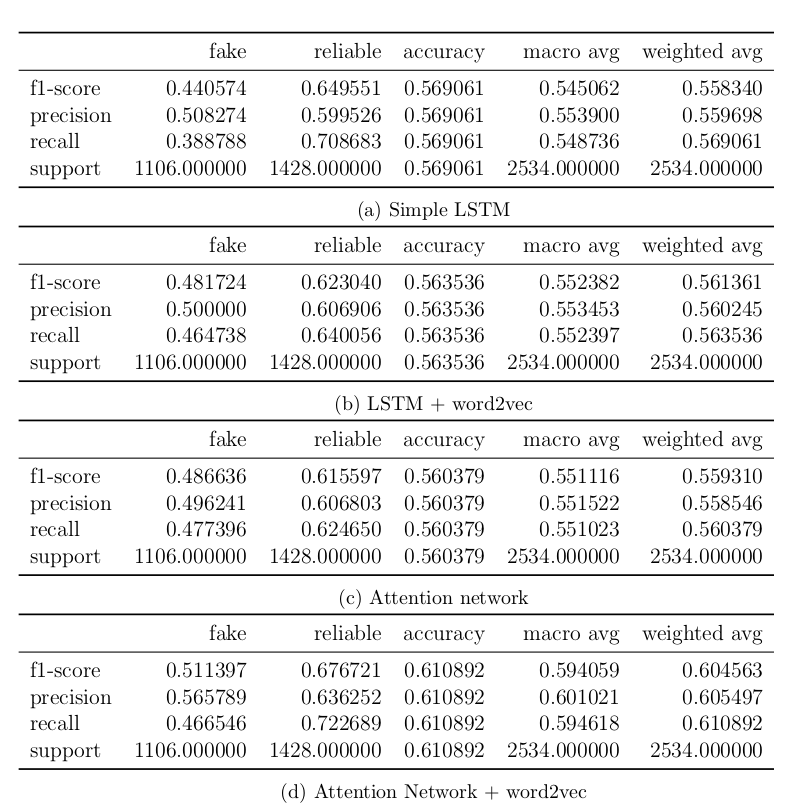
\includegraphics[width=0.6\textwidth]{res4.png}
		\end{figure}
	\end{frame}
	\begin{frame}{Fake news corpus results}
		\begin{figure}
		\centering
			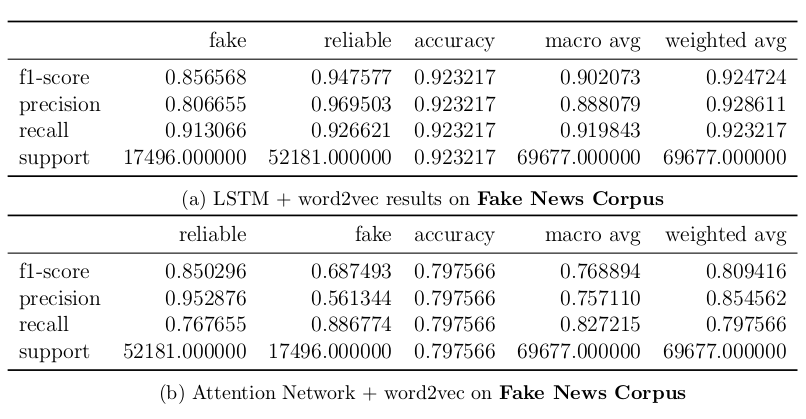
\includegraphics[width=0.8\textwidth]{res5.png}
		\end{figure}
		\note{Comparer aux $93\%$ et $94\%$ pour SVM et ridge classifier}
	\end{frame}
	\begin{frame}{Conclusion}
		\begin{itemize}
			\item Attention Mechanism and LSTMs does not impove results
			\item Using only text content for liar-liar corpus is not enougth
			\item Very good results on fake news corpus.
		\end{itemize}
	\end{frame}
  \begin{frame}[allowframebreaks]{Bibliography}
    \bibliographystyle{unsrt}
	\bibliography{../references/references.bib}
	\note{}
  \end{frame}
\end{document}